\documentclass[aspectratio=169]{beamer} % for making videos 169 is inferior
\usepackage{graphicx}
\usepackage[utf8]{inputenc}

\usetheme{AnnArbor}
\usecolortheme{XKDR}
\logo{
\includegraphics[width=1cm]{XKDR_Logomark_RGB_Full_Colour.png}}

\hypersetup{colorlinks,
    citecolor=blue,
    linkcolor=blue,
    anchorcolor=yellow
    }

\mode<presentation>
{
  \usetheme{boxes}
}

\usepackage[english]{babel}
% \usepackage[latin1]{inputenc}
\usepackage{times}
\usepackage[T1]{fontenc}

\newcommand{\fullpage}[1]{
  \begin{frame}
    \vfill
    {\Large #1}
    \vfill
  \end{frame}
}

\addtobeamertemplate{navigation symbols}{}{%
    \usebeamerfont{footline}%
    \usebeamercolor[fg]{footline}%
    \hspace{1em}%
    {\large \insertframenumber/\inserttotalframenumber}
}

\usepackage[style=apa, citestyle=authoryear, bibstyle=numeric, natbib=true, backend=biber]{biblatex}
\addbibresource{regbibliography.bib}

\title{The unreasonable effectiveness of Julia}
\titlegraphic{
\includegraphics[width=2.88cm]{XKDR_Primary_Logo_RGB_Full_Colour.png}}
\author{Ayush Patnaik}

\hypersetup{pdfauthor   = Ayush Patnaik,
            pdftitle    = The unreasonable effectiveness of Julia,
            pdfsubject  = Julia effectiveness, 
            pdfkeywords = {Julia}
}

\begin{document}

\begin{frame}
  \titlepage
\end{frame}

\section{Motivation}

\begin{frame}{Motivation for Julia}
  Julia was born out of addressing the limitations of MATLAB, Python, R and other high-level languages. 
  \begin{enumerate}
    \item To produce performant code in the existing frameworks, one had to resort to writing the heavy lifting code in other languages or opt for other ``inelegant'' solutions. 
    \item The existing scientific computing languages had proprietary code, limiting accessibility to their source code and imposing restrictions on customization and collaborative development.
  \end{enumerate}
  To replace the existing framework, Julia needed to be significantly better in terms of elegance, performance, and fostering a collaborative ecosystem. This became the core culture of Julia.  
\end{frame}

\begin{frame}
  \frametitle{JIT Compilation in Julia}

  \begin{itemize}
    \item \textbf{JIT Compilation:} Compiles code at runtime for efficient execution.
    \item \textbf{LLVM Backend:} Generates machine code optimized for the target CPU.
    % \item \textbf{Steps:}
    %   \begin{enumerate}
    %     \item \textbf{Parsing \& Type Inference:} Determines types at runtime.
    %     \item \textbf{Code Generation:} Creates specialized machine code for types.
    %     \item \textbf{Execution:} Runs optimized machine code, reusing previous compilations.
    %   \end{enumerate}
    \item \textbf{Performance:} 
      \begin{itemize}
        \item Speeds up execution to near C-level performance.
        \item Dynamic typing with high efficiency.
      \end{itemize}
  \end{itemize}
  
\end{frame}

\begin{frame}[fragile]
  \frametitle{LLVM}

  Consider the function \verb|f(x) = 5x^2 + 3x + 8|. The corresponding LLVM Intermediate Representation (IR) for this function is:
  \scriptsize
  \begin{verbatim}
define i64 @julia_f_1090(i64 signext %0) #0 {
top:
; @ int.jl:88 within `*`
  %1 = mul i64 %0, 5               ; Multiply the input value (%0) by 5. 
  %reass.add = add i64 %1, 3       ; Add 3 to the result of the multiplication.
  %reass.mul = mul i64 %reass.add, %0 ; Multiply (5x + 3) by the input value (%0).
; 
; @ operators.jl:587 within `+` @ int.jl:87
  %2 = add i64 %reass.mul, 8       ; Add 8 to the result.  
  ret i64 %2                       ; Return the final result as a 64-bit integer.
; 
  }
  \end{verbatim}
\normalsize
\end{frame}

\begin{frame}[fragile]
  \frametitle{Native of the same function}
  When the function is compiled the following assembly code is generated:

  \scriptsize
  \begin{verbatim}
.type julia_f_1092,@function
julia_f_1092:                          # @julia_f_1092
; @ REPL[53]:1 within `f`
# %bb.0:                               # %top
  push  rbp                            ; Save the base pointer (set up stack frame)
  mov   rbp, rsp                       ; Set the base pointer to the current stack pointer

  lea   rax, [rdi + 4*rdi]             ; Compute rdi * 5 (5x). rdi holds the input x.
  add   rax, 3                         ; Add 3 to the result of rdi * 5 (5x + 3)
  imul  rax, rdi                       ; Multiply the result by rdi (x * (5x + 3))

; @ operators.jl:587 within `+` @ int.jl:87
  add   rax, 8                         ; Add 8 to the result (5x^2 + 3x + 8)

  pop   rbp                            ; Restore the base pointer 
  ret                                  ; Return the final result in rax
.Lfunc_end0:
  .size julia_f_1092, .Lfunc_end0-julia_f_1092  ; Size of the function
; -- End function
  \end{verbatim}
  \normalsize

\end{frame}

\begin{frame}
  \frametitle{The Two-Language Problem}
  \begin{itemize}
    \item The two-language problem refers to the need to use two different programming languages in scientific computing and data analysis:
      \begin{itemize}
        \item A high-level language (e.g., Python, R) for ease of use and rapid development.
        \item A low-level language (e.g., C, Fortran) for performance-critical tasks.
      \end{itemize}
    \item This approach has several drawbacks:
      \begin{itemize}
        \item Increased complexity in code maintenance and development.
        \item Difficulty in debugging and profiling across language boundaries.
        \item Potential for errors and inefficiencies in the interface between the two languages.
      \end{itemize}
    \item Julia aims to solve the two-language problem by providing:
      \begin{itemize}
        \item High-level syntax and ease of use similar to Python and R.
        \item Performance comparable to low-level languages like C and Fortran.
        \item A single language for both prototyping and production code.
      \end{itemize}
  \end{itemize}
\end{frame}

\begin{frame}[fragile]
  \frametitle{Example of the two language problem}
  \framesubtitle{tsoutliers in R using supsmu from FORTRAN} 
  \begin{center}
    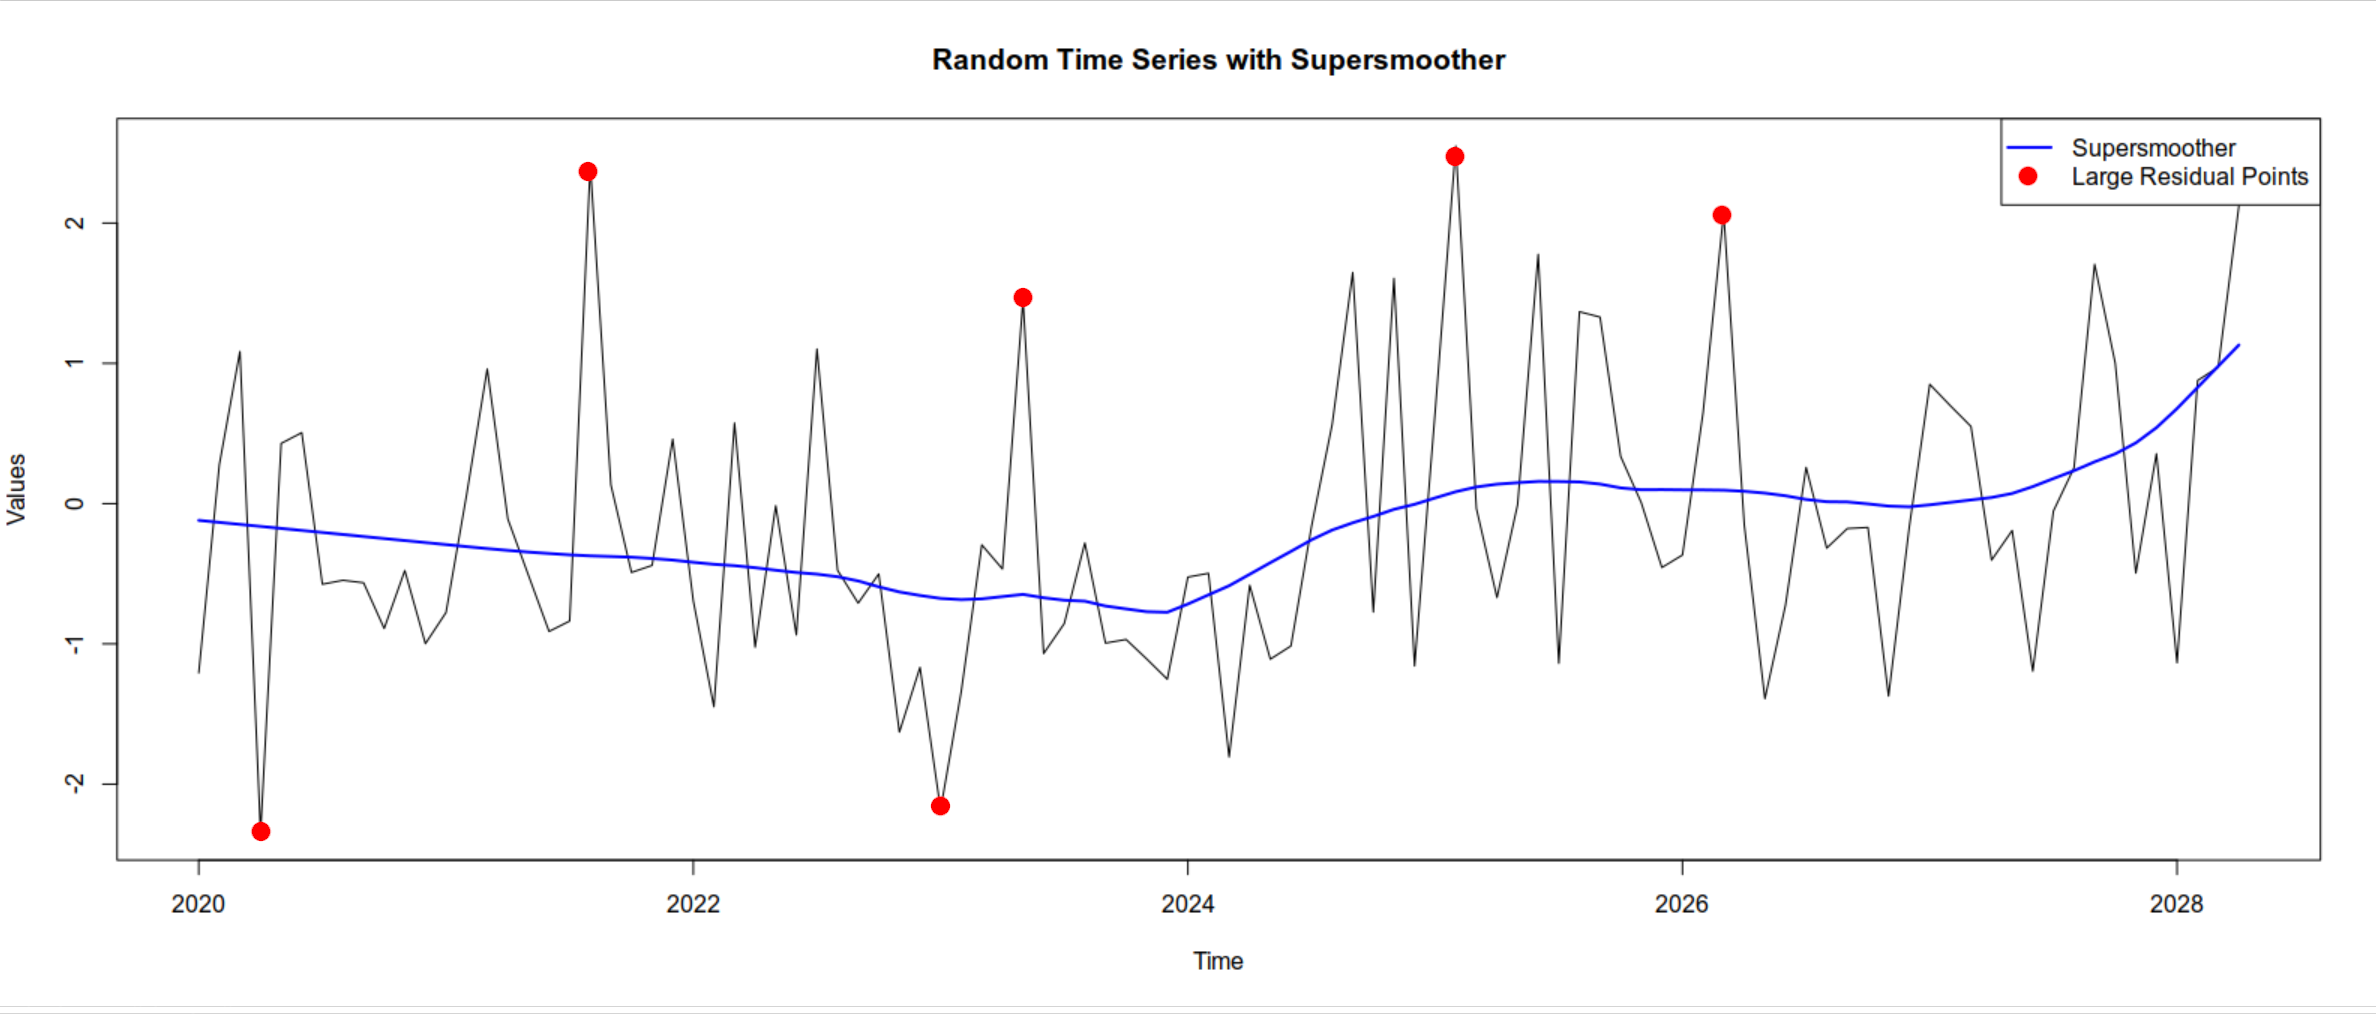
\includegraphics[width=0.7\linewidth]{time_series.png}
  \end{center}

  \begin{columns}

    \column{0.2\textwidth}

    \scriptsize
    \begin{verbatim}
tt <- 1:n
mod <- supsmu(tt, xx)
resid <- xx - mod$y
    \end{verbatim}
    \normalsize

    \column{0.8\textwidth}

    \scriptsize
    \begin{verbatim}
    resid.q <- quantile(resid, probs = c(0.25, 0.75), na.rm = TRUE)
    iqr <- diff(resid.q)
    limits <- resid.q + 3 * iqr * c(-1, 1)
    # Find residuals outside limits
    if ((limits[2] - limits[1]) > 1e-14) {
      outliers <- which((resid < limits[1]) | (resid > limits[2]))
    } 
    \end{verbatim}
    \normalsize
  \end{columns}

  \vfill
  \footnotesize
  \href{https://github.com/robjhyndman/forecast/blob/0583d2fef45336ee59ef486e24b356520350da9a/R/clean.R#L208}{robjhyndman/forecast/clean.R line 208}
\end{frame}
\begin{frame}[fragile]
  \frametitle{Supsmu Subroutine}
  The \verb|supsmu| subroutine is used for smoothing data. Here is an excerpt from the 130 line FORTRAN code:

  \scriptsize
  \begin{verbatim}
      subroutine smooth (n,x,y,w,span,iper,vsmlsq,smo,acvr)
      dimension x(n),y(n),w(n),smo(n),acvr(n)
      integer in,out
      double precision wt,fbo,fbw,xm,ym,tmp,var,cvar,a,h,sy
      xm=0.0
      ym=xm
      var=ym
      cvar=var
      fbw=cvar
      jper=iabs(iper)
      ibw=0.5*span*n+0.5
      if (ibw.lt.2) ibw=2
      it=2*ibw+1
      do 20 i=1,it
  \end{verbatim}
  \normalsize

  \vfill
  \footnotesize
  For more details, refer to the following GitHub link: \href{https://github.com/jakevdp/supsmu/blob/master/supsmu/_supsmu.f}{GitHub Reference}

  \vfill
  \footnotesize
  \textit{Coded and copyright (c) 1984 by: Jerome H. Friedman, Department of Statistics and Stanford Linear Accelerator Center, Stanford University}
\end{frame}

\begin{frame}
  \frametitle{The Cathedral and the Bazaar}

  \begin{itemize}
    \item The Cathedral model:
      \begin{itemize}
        \item Software is developed by a small group of developers.
        \item Code is released only when it is fully developed.
        \item Limited external contributions.
      \end{itemize}
    \item The Bazaar model:
      \begin{itemize}
        \item Software is developed in the open with many contributors.
        \item Code is released early and often.
        \item Encourages external contributions and collaboration.
      \end{itemize}
  \end{itemize}

  \vspace{0.5cm}

  \textbf{Why the Bazaar model is better:}
  \begin{itemize}
    \item Superior code quality due to many eyes on it.
    \item Faster identification and fixing of bugs.
    \item Diverse perspectives lead to innovative solutions.
    \item Encourages a collaborative and inclusive development environment.
  \end{itemize}
\end{frame}

\begin{frame}
  \frametitle{Creating a Julia Package}

  On the very first day, you put the package on GitHub. People start contributing through Pull Requests (PRs), and there are Continuous Integration (CI) tests to ensure code quality and functionality. For example, Survey.jl has benefited greatly from community contributions, with many contributors improving the package through PRs and CI tests.

  \begin{table}[]
    \centering
    \scriptsize
    \begin{tabular}{|c|c|c|c|c|}
      \hline
      \textbf{Rank} & \textbf{Contributor} & \textbf{Commits} & \textbf{Additions} & \textbf{Deletions} \\ \hline
      1 & ayushpatnaikgit & 199 & 11,736 & 4,276 \\ \hline
      2 & iuliadmtru & 197 & 33,544 & 3,788 \\ \hline
      3 & smishr & 171 & 7,682 & 8,535 \\ \hline
      4 & nadiaenh & 51 & 1,259 & 626 \\ \hline
      5 & codetalker7 & 50 & 818 & 312 \\ \hline
      6 & harsharora21 & 22 & 2,607 & 58 \\ \hline
      7 & sayantikaSSG & 13 & 424 & 221 \\ \hline
      8 & greimel & 10 & 86 & 91 \\ \hline
      9 & asinghvi17 & 7 & 17 & 10 \\ \hline
      10 & itsdebartha & 5 & 16 & 6 \\ \hline
      11 & jishnub & 2 & 26 & 16 \\ \hline
    \end{tabular}
    \caption{Top contributors to Survey.jl}
  \end{table}

\end{frame}


\begin{frame}
  \frametitle{Slow and steady}

  Julia development can be slow sometimes, but the quality is much better. Here is an example of a pull request for the GLM package:

  \begin{center}
    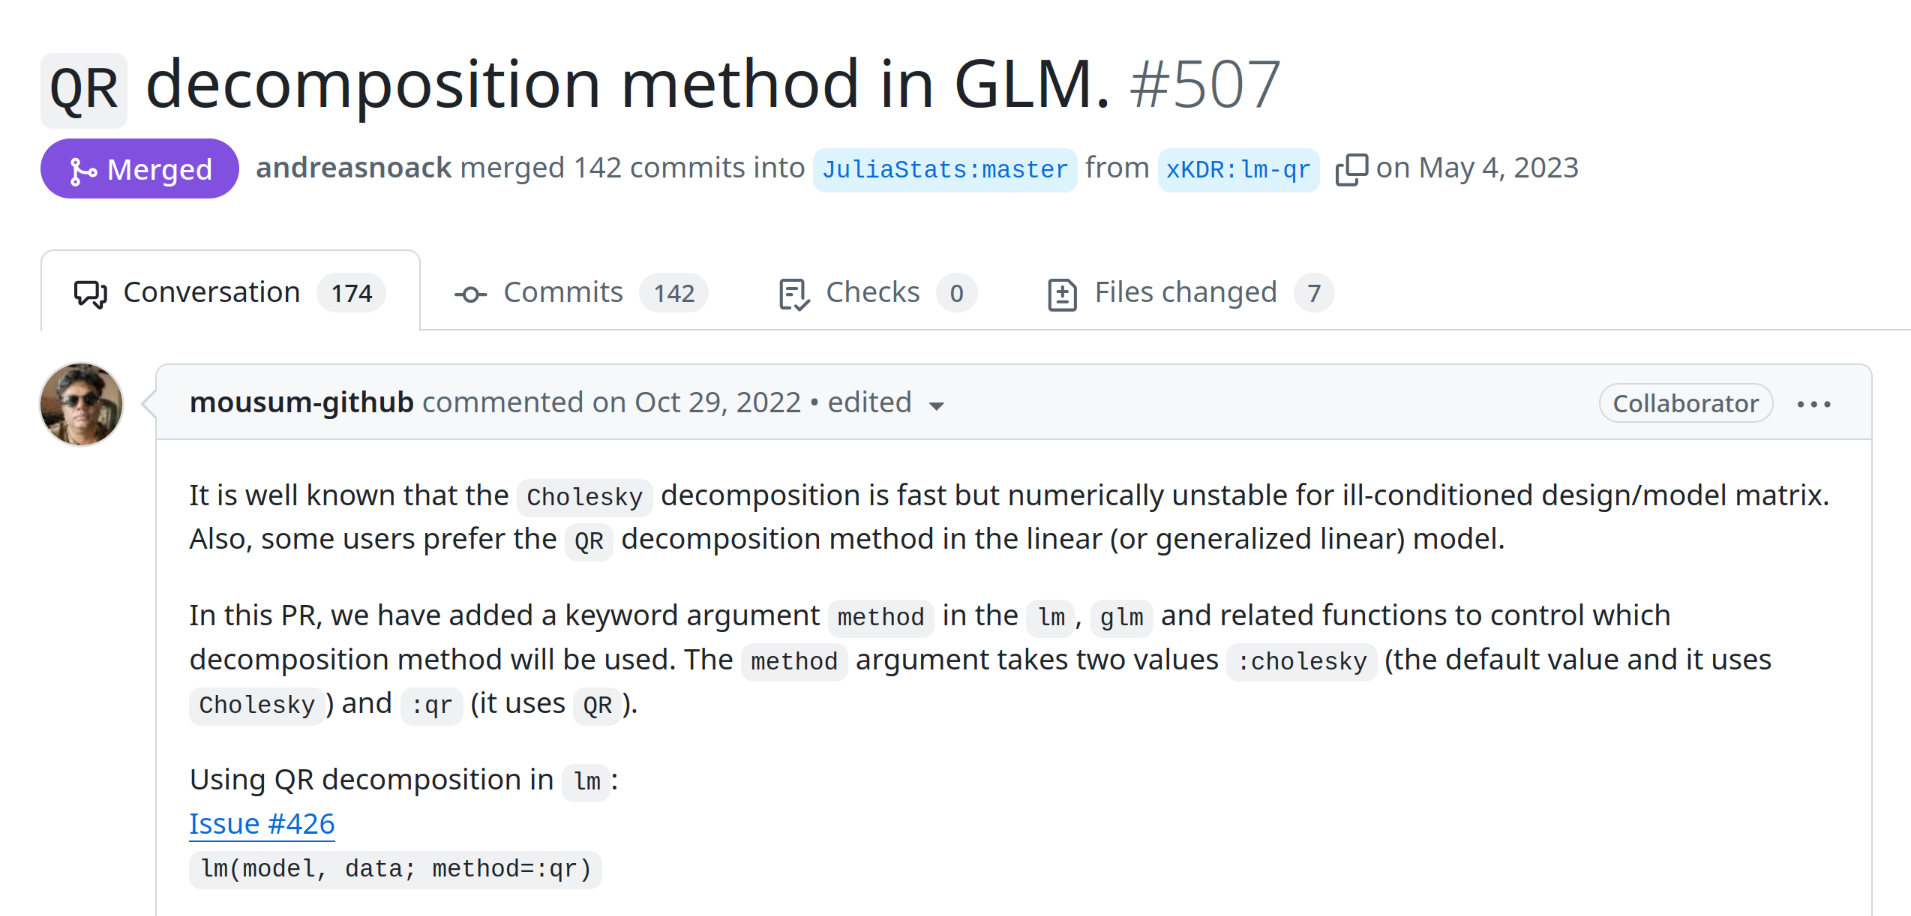
\includegraphics[width=0.7\linewidth]{GLM_PR.png}
  \end{center}

  \vfill
  \footnotesize
 
  The thorough review process ensures high-quality contributions.
\end{frame}

\begin{frame}
  \frametitle{Julia Packages Covered Today}

  \begin{description}
    \item[Turing.jl] Probabilistic programming library for Julia.
      \begin{itemize}
        \item Allows for flexible and efficient Bayesian inference.
        \item Integrates seamlessly with Julia's ecosystem.
        \item Simplifies complex statistical modeling and inference, making it accessible to a wider audience.
      \end{itemize}
    \item[Flux.jl] Machine learning library for Julia.
      \begin{itemize}
        \item Provides a simple and intuitive API for building neural networks.
        \item Combines ease of use with high performance, enabling rapid experimentation and deployment of machine learning models.
      \end{itemize}
  \end{description}
  These are made possible by Julia's ability to perform automatic differentiation (AD).
\end{frame}

\begin{frame}[fragile]
  \frametitle{Automatic Differentiation}

  Using \verb|Zygote.jl| to calculate the derivative of the function \verb|f(x) = 5x^2 + 3x|:

  \scriptsize
  \begin{verbatim}
  using Zygote
  f(x) = 5x^2 + 3x
  df(x) = Zygote.gradient(f, x)[1]
  \end{verbatim}
  \normalsize

  The corresponding LLVM Intermediate Representation (IR) for the derivative calculation is:

  \scriptsize
  \begin{verbatim}
  %1 = shl i64 %0, 1              # Compute 2 * x (via left shift)
  %2 = sitofp i64 %1 to double    # Convert integer to float for floating-point operations
  %3 = fmul double %2, 5.000000e+00 # Compute 10 * x
  %4 = fadd double %3, 3.000000e+00 # Add 3 to 10 * x
  ret double %4                   # Return the result (10 * x + 3)
  \end{verbatim}
  \normalsize

\end{frame}

\begin{frame}
  \vfill
  \centering {\LARGE Getting started}

  \vfill

\end{frame}

\begin{frame}[fragile]
  \frametitle{Installation}
  Julia multiplexer gets installed with just a single command. No \verb|sudo| required.  
  \begin{verbatim}
    curl -fsSL https://install.julialang.org | sh
  \end{verbatim}

  Everything is in the \verb|.julia| folder. 
  \begin{verbatim}
    ayush@woodpecker:~/.julia$ ls
    artifacts  environments  logs      registries
    compiled   juliaup       packages  scratchspaces
  \end{verbatim}

\end{frame}

\begin{frame}[fragile]
  \frametitle{Syntax}
  
  \begin{columns}[t]
  \column{0.5\textwidth}
  Variable declaration
  \begin{verbatim}
  a = 10
  b = 20
\end{verbatim}

Arithmetic operations
\begin{verbatim}
  sum = a + b
  product = a * b
\end{verbatim}
Conditional statement
\begin{verbatim}
  age = 25
  if age >= 18
    println("You're an adult.")
  else
    println("You're a minor.")
  end
  \end{verbatim}
  
  \column{0.5\textwidth}
  Define a function
  \begin{verbatim}
  function greet(name)
    println("Hello ", name)
  end
\end{verbatim}
Call the function
\begin{verbatim}
  greet("Julia")
\end{verbatim}
Array creation
\begin{verbatim}
  numbers = [1, 2, 3, 4, 5]
\end{verbatim}
Loop through elements  
\begin{verbatim}
  for num in numbers
    println(num)
  end
  \end{verbatim}
  \end{columns}
  
  \end{frame}
%%%%%%%%%
  \begin{frame}[fragile]
    \frametitle{Syntax}
    \framesubtitle{Continued}

    \begin{columns}[t]
    \column{0.5\textwidth}
    List comprehension
    \begin{verbatim}
  squares = [i^2 for i in 1:5]
  squares = [i^2 for i in numbers]
  \end{verbatim}
  
  Dictionary creation
  \begin{verbatim}
  person = Dict(
  "name" => "Alice",
  "age" => 30,
  "city" => "New York")
  \end{verbatim}
  Access values by key
  \begin{verbatim}
  person["name"])
    \end{verbatim}
    
    \column{0.5\textwidth}
  Create a matrix
\begin{verbatim}
  A = [1 2 3; 4 5 6; 7 8 9]
\end{verbatim}
Basic indexing
\begin{verbatim}
  element = A[2, 3]
  second_row = A[2, :]
  third_column = A[:, 3]
  submatrix = A[1:2, 2:3] 
\end{verbatim}
    Broadcasting example
    \begin{verbatim}
  A = [1 2 3; 4 5 6; 7 8 9]
  B = [2 2 2; 2 2 2; 2 2 2]
  C = A .+ B
  \end{verbatim}
    \end{columns}
    
    \end{frame}


\begin{frame}[fragile]
    \frametitle{Multiple Dispatch}
    \framesubtitle{Methods are selected based on all argument types}
    
    \begin{columns}[t]
        \column{0.5\textwidth}
        Define methods for different types
        \begin{verbatim}
function process(x::Number,
                 y::Number)
    return x + y
end

function process(x::String,
                 y::String)
    return x * y
end

function process(x::Array,
                 y::Array)
    return x .+ y
end
        \end{verbatim}

        \column{0.5\textwidth}
        Julia automatically selects correct method
        \begin{verbatim}
process(1, 2)         # 3
process("a", "b")     # "ab"
process([1,2], [3,4]) # [4,6]
        \end{verbatim}

        \vspace{0.3cm}
        \begin{itemize}
            \item No explicit method overloading needed
            \item Dispatch based on all arguments
            \item Compiler optimizes for each type combination
        \end{itemize}

    \end{columns}
    

\end{frame}

\begin{frame}[fragile]
    \frametitle{Multiple Dispatch in action}
    \framesubtitle{Same plot() function, different types}
    
    \begin{columns}[t]
        \column{0.48\textwidth}
        Vector plotting
        \begin{verbatim}
  using Plots
  x = range(0, 10, length=100)
  y = sin.(x)
  plot(x, y) 
        \end{verbatim}
        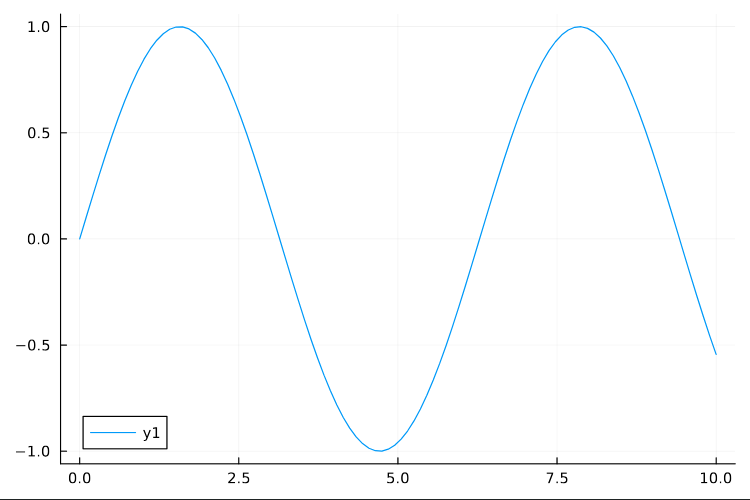
\includegraphics[width=0.8\textwidth]{sin_plot.png}
        
        \column{0.48\textwidth}
        Raster plotting
        \begin{verbatim}
  using Rasters
  A = Raster(WorldClim{BioClim},
             5)
  plot(A) 
        \end{verbatim}
        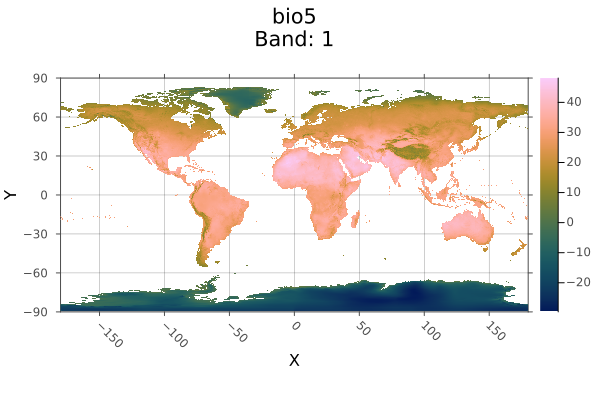
\includegraphics[width=0.9\textwidth]{raster_plot.png}
    \end{columns}
    
    \vspace{0.2cm}
    \begin{itemize}
        \item Same plot() function handles different types
        \item No explicit method selection needed
        \item Automatic dispatch to appropriate visualization
    \end{itemize}
\end{frame}

\begin{frame}[fragile]
  \frametitle{Using macros in Julia}

  Measuring execution time with \verb|@time|
  \begin{verbatim}
  @time sum(1:1000000)
  \end{verbatim}

  Benchmarking with \verb|@btime|
  \begin{verbatim}
  using BenchmarkTools
  @btime sin(1.0)
  \end{verbatim}

  Displaying variable values with \verb|@show|
  \begin{verbatim}
  x = 42
  @show x
  \end{verbatim}

\end{frame}


\begin{frame}[fragile]
  \frametitle{Package manager which doesn't fail}
  \vspace{0.5cm}  
  \begin{columns}[t]
  \column{0.5\textwidth}
  Adding a package
  \begin{verbatim}
  using Pkg
  Pkg.add("ExamplePackage")
  \end{verbatim}
  Updating packages
  \begin{verbatim}
  Pkg.update()
  \end{verbatim}
  \column{0.5\textwidth}
  Removing a package
  \begin{verbatim}
  Pkg.rm("ExamplePackage")
  \end{verbatim}
  Listing installed packages
  \begin{verbatim}
  Pkg.status()
  \end{verbatim}
  \end{columns}
\end{frame} 


\begin{frame}
  \hfill {\LARGE Thank you}.

  \vfill
  \vfill

  \hfill \url{https://xkdr.org}
\end{frame}


\end{document}
